\chapter{Frameworks}
\label{cap:Frameworks}

\section{Natural Language Toolkit}

O \ac{NLTK} é um \textit{Framework} para Python
criado em 2001 na Universidade de Pensilvânia. Ele contém mais de 50 dicionários
e modelos já treinados incluindo:

\begin{itemize}
  \item \textit{Sentiment Polarity Dataset Version 2.0} - Conjunto de dados já
  classificados que contém mais de 1000 filmes avaliados de forma positiva e
  1000 filmes avaliados de forma negativa.
  \item \textit{SentiWordNet} - Provém um dicionário com as palavras extraídas
  do WordNet já classificadas em positividade, negatividade e objetividade.
  \item \textit{VADER Sentiment Lexicon} - Dicionário especificamente ajustado
  para análise de sentimentos expressos em mídias sociais.
\end{itemize}


\subsection{Análise de Sentimentos}

Para a análise de sentimentos, o \ac{NLTK} já possui implementado as dois
classificadores citados anteriormente, \textit{Naive Bayes} e também
\ac{MaxEnt}.

Podemos utilizar o classificador Naive Bayes a partir da classe

\textbf{nltk.classify.naivebayes.NaiveBayesClassifier} através dos seguintes métodos:

\begin{itemize}
  \item \textit{classify(featureset)} - Classifica a partir de um conjunto de
  atributos.
  \item \textit{most\_informative\_features(n=100)} - A partir de um
  classificador treinado, retorna os atributos mais relevantes.
  \item \textit{train(trainingset)} - Treina um classificador a partir de um \textit{training set}.
\end{itemize}

Podemos utilizar o classificador \ac{MaxEnt} a partir do módulo
\textbf{nltk.classify.maxent} através dos seguintes métodos:

\begin{itemize}
  \item \textit{train(train\_toks, algorithm=None, trace=3,
  encoding=None, labels=None, gaussian\_prior\_sigma=0, **cutoffs)} - Treina um
  classificador \ac{MaxEnt} a partir de um \textit{training set}.
  \begin{itemize}
    \item \textit{train\_toks} - \textit{Training set}.
  \item \textit{algorithm} - Algorítmo a ser usado para treinar o classificador. 
%   Pode receber: \textit{Generalized Iterative Scaling ('GIS')}, \textit{Improved
%   Iterative Scaling ('IIS')} ou LM-BFGS ('megam'). O algorítmo utilizado
%   por padrão é IIS.
  \item \textit{trace} - Nível de detalhe utilizado no log.
  \item \textit{encoding}
  \item \textit{labels} - Uma lista de possíveis rótulos, se nenhuma for
  especificada, todos os labels do \textit{training set} serão utilizados.
  \item \textit{gaussian\_prior\_sigma=0} - Somente utilizado no LM-BFGS.
  \item \textit{cutoffs} - Argumentos que especificam condições em que o
  processo será terminado.
  \end{itemize}
\item \textit{classify(featureset)} - Classifica a partir de um conjunto de
  atributos.
\item \textit{explain(featureset, columns=4)} - Mostra uma tabela demonstrando
os efetiso de cada atributo e como eles combinam para determinar a probabilidade
de cada rótulo.
\item \textit{show\_most\_informative\_features(n=10, show='all')} - A partir de
um classificador treinado, retorna os atributos mais relevantes.
\end{itemize}

Ele também contém um pacote contendo classes úteis para a análise de sentimentos
chamado de \textit{nltk.sentiment}. Nesse pacote temos os seguintes módulos:


\begin{itemize}
  \item Classe \textit{nltk.sentiment.sentiment\_analyzer.SentimentAnalyzer} -
  Ferramentas para facilitar e implementar análise de sentimentos,
  especialmente para demonstrações e ensino.
  \item Módulo \textit{nltk.sentiment.util} - Contém diversas classes de
  demonstrações e utilitários como conversão de \textit{json} para \textit{csv}.
  \item Módulo \textit{nltk.sentiment.vader} - Ferramenta de Análise VADER.
\end{itemize}

\section{Stanford CoreNLP}

O Stanford CoreNLP é um conjunto de ferramentas escrito em Java para
processamento de linguagem natural. Dentre essas ferramentas, estão incluídos:
\textit{Part-of-Speech Tagging} ou classificação gramatical, reconhecimento de
entidade e análise de sentimentos. Também possui suporte a diversas linguas além
do inglês, como: árabe, chinês, francês, alemão e espanhol.

\subsection{Análise de Sentimentos}

A análise de sentimentos do Stanford CoreNLP é realizada através de um novo
modelo de rede neural construído em cima de estruturas gramaticais chamado de
\ac{RNTN}. Seu modelo é treinado a partir do \textit{Sentiment Treebank}, um
banco de dados que possui 215.154 orações distribuidas em 11.855 árvores de
frases com sentimentos já classificados.

\begin{figure}[htbp]
 \centering
 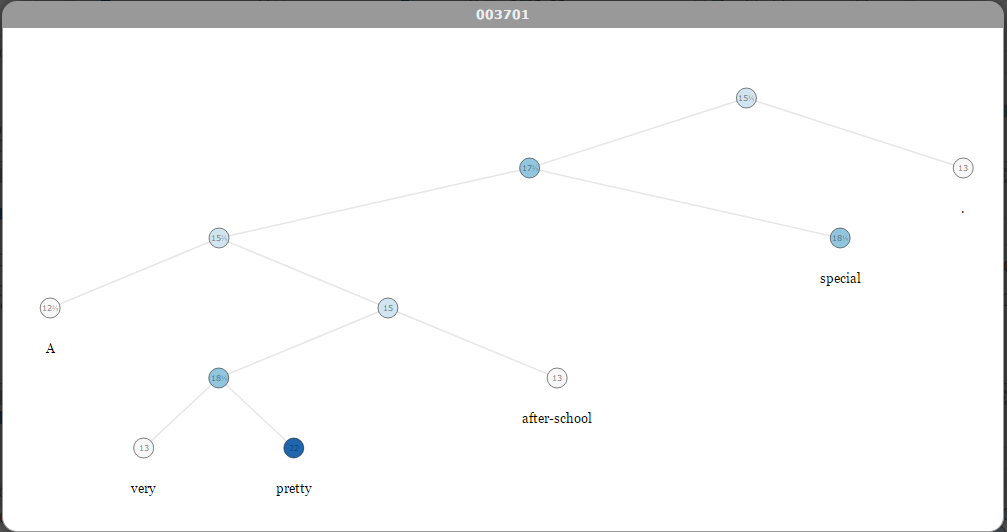
\includegraphics[height=225px]{imagens/corenlp.png}
 \caption{Frase já classificada disponível no Sentiment Treebank}
 \label{fig:corenlp}
\end{figure}

A sua utilização pode ser feita de diversas formas, como linha de comando,
através de um servidor \textit{web} e através de sua API java:


\begin{figure}[htbp]
 \centering
 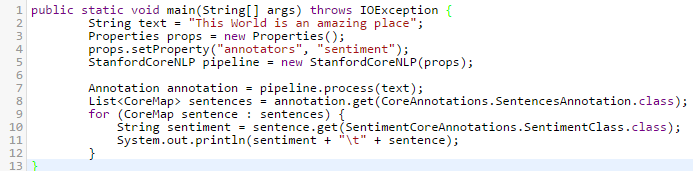
\includegraphics[height=120px]{imagens/corenlp1.png}
 \caption{Exemplo de implementação}
 \label{fig:corenlp}
\end{figure}

Como resultado, o console java irá imprimir que a frase é muito positiva ou
\textit{Very positive}.

